\chapter{Arsitektur Client-Server}
\authors{Alfa Yohannis}

\section{Latar Belakang}
Pada awal komputer bermula sebagai suatu kesatuan, tidak terpisah-pisah. Perangkat lunak hanya berjalan pada satu unit komputer tersebut. Secara perlahan, ada bagian komputer yang dapat terpisah secara fisik dan menjalankan tanggung jawab tertentu. Sebagai contoh, data storage terpisah dari komputer utama. Lalu, beberapa fungsionalitas akhirnya terpisah dan membutuhkan mesin tersendiri. Misalnya, komputer yang didedikasikan untuk menyimpan data atau yang kita sebut sebagai \textit{database server}. Di sisi lain, jaringan komputer juga berkembang dan kemudian menjadi sesautu yang umum. Komputer-komputer saling berkomunikasi satu sama yang lain, dan setiap komputer dapat memiliki peran-peran tertentu yang memungkinkan lahirnya sistem terdistribusi.

\section{Arsitektur Client-Server}
Suatu sistem \textit{client-server} terdiri dari satu \textit{server} dan satu \textit{client} atau lebih. \textit{Server} biasanya memiliki kemampuan komputasi dan penyimpanan data yang lebih cepat dan banyak dibanding \textit{client}. Oleh karena itu, \textit{client} menugaskan \textit{server} untuk melakukan komputasi tertentu dan menerima hasilnya atau sekedar menarik data dari \textit{server}.

Terdapat 2 jenis \textit{client-server architecture}: \textit{two-tier architecture} dan \textit{three-tier architecture}. Two tier-architecture umumnya hanya terdiri dari \textit{desktop application} yang berada di sisi klien dan \textit{database} yang berada di sisi server. Contoh lain adalah \textit{web browser} yang memuat \textit{web application} dan \textit{web server} untuk melakukan \textit{backend computation}.
Arsitektur tersebut dapat diperluas menjadi \textit{three-tier architecture}, dengan menambahkan \textit{database server} seperti yang ditampilkan pada Gambar \ref{fig:client-server-schema}.

\begin{figure}[h]
    \centering
    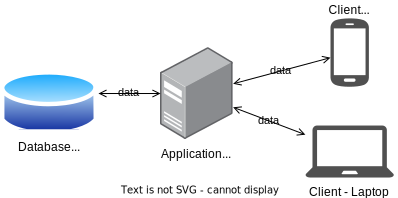
\includegraphics[width=\textwidth]{client-server-3-tier}
    \caption{Skema dari 3-tier client-server arsitektur.}
    \label{fig:client-server-schema}
\end{figure}

\section{Kelebihan dan Kekurangan}
Berikut adalah kelebihan dan kekurangan arsitektur client-server:

\subsection{Kelebihan}
Keuntungan dari menerapkan arsitektur client-server adalah:
\begin{itemize}
\item Kemampuan komputasi (dan penyimpanan data) dapat diakses dari berbagai lokasi berjauhan dan oleh banyak komputer/pengguna.
\item Komputasi-komputasi yang membutuhkan kinerja tinggi dapat didelegasikan ke server.
\item Data dapat disentralisasikan sehingga meningkatkan konsistensi data dan mengurangi duplikasi data.
\item  Sistem dapat menerapkan \textit{horizontal scaling }untuk skalabilitas. Horizontal scaling adalah meningkatkan kinerja komputer dengan penambahan komputer agar beban komputasi dibagi ke komputer-komputer yang tersedia. Misalnya, awalnya terdapat 10 000 requests perhari yang ditangani oleh suatu \textit{application server}. Jika \textit{application server} ditambah, maka beban tersebut dibagi di antara kedua \textit{server} tersebut. Vertical scaling adalah meningkat kinerja suatu komputer dengan menaikkan spefikasi komputer tersebut, misalnya dengan menggunakan prosesor yang lebih cepat atau meningkatkan kapasitas memori.
\end{itemize}

\subsection{Kekurangan}
Konsekuensi dari penerapan arsitektur client-server adalah sistem jadi lebih kompleks untuk dikelola:
\begin{itemize}
\item Biaya akan meningkat karena terdapat komponen/mesin tambahan yang perlu dikelola.
\item Faktor keamanan juga perlu diperhatikan karena server dan client beroperasi dalam suatu jaringan komputer yang mana rawan terhadap \textit{cyber attack}.
\item Perlunya koordinasi antar-komputer, misalnya komunikasi sinkron dan asinkron serta komputasi parallel.
\item Kompatibilitas antara \textit{server} dan \textit{client} maupun sesama klien.
\item Masalah-masalah yang umum terdapat pada jaringan komputer etwork problems, misalnya \textit{network latency}, kesalahan dalam konfigurasi jaringan, dsb.
\end{itemize}

\section{Contoh Kasus}

\subsection{Deskripsi}
Jelaskan contoh kasus yang dipaparkan berkaitan dengan arsitektur yang dimaksud pada bab ini.
Contoh kasus harus memperjelas arsitektur yang dimaksud.

\subsection{Penjelasan Implementasi}
Jelaskan bagian-bagian kode program, basisdata, atau konfigurasi yang signifikan terhadap arsitektur yang dimaksud.

\section{Kesimpulan}
Rangkum dan ulangi (beri penekanan pada) hal-hal kunci dari arsitektur yang dimaksud.